\documentclass[12pt]{article}

\setlength{\parskip}{1em}

\usepackage[frenchb]{babel}
\usepackage[T1]{fontenc}
\usepackage{times}
\usepackage[utf8]{inputenc}
\usepackage{amsmath}
\usepackage{textcomp}
\usepackage{mathtools}
\usepackage{arevmath}
\usepackage{amsfonts}
\usepackage{slantsc}
\usepackage{xcolor}
\usepackage{graphicx}
\usepackage[a4paper, margin=1in]{geometry}

\usepackage{hyperref}
\hypersetup{
  colorlinks=true,
  linkcolor=blue,
  urlcolor=blue,
  pdftitle={LO21 Projet: BOZANE ESTEBAN}
}

\usepackage{listings}
\lstset{
  numbers=left,
  columns=fullflexible,
  language=C,
  numberstyle=\scriptsize,
}

\usepackage[linesnumbered, french]{algorithm2e}
\SetKwInput{Data}{Donn\'ees}
\SetKwInput{Result}{R\'esultat}
\SetKwInput{Vars}{Variables}
\SetKwInput{Assertion}{Assertion}
\SetKwIF{If}{ElseIf}{Else}{Si}{alors}{Sinon si}{Sinon}{FinSi}
\SetKwFor{While}{Tant que}{faire}{Fin TantQue}
\SetKwBlock{Begin}{D\'ebut}{Fin}
\SetKwRepeat{Repeat}{Faire}{Tant que}
\DontPrintSemicolon
\SetAlgoLined

\RestyleAlgo{boxruled}

\newcommand{\Assign}[2]{#1 $\; \longleftarrow \;$ #2}
\newcommand{\Arg}[2]{\hspace{0.2em}#1\hspace{0.05em}: #2}
\newcommand{\Child}[2]{#2(#1)}
\newcommand{\Null}[0]{\textsc{null}\hspace{4pt}}
\newcommand{\Et}[2]{#1\hspace{2pt}\textnormal{\textbf{et}}\hspace{2.5pt}#2}
\newcommand{\Not}[1]{\textnormal{\textbf{non}}(#1)}

\begin{document}

\title{LO21}
\author{Marius Bozane\\
Louis Esteban
}
\date {Automne 2020}
\maketitle

\begin{abstract}
	Pour notre projet de LO21 nous devions réaliser un système expert composé de bases de connaissances, de règles et d'un moteur d'inférence.\\
	\\	
	Une règle est composé d'une prémisse et d'une conclusion\\
	\\
	Les règles sont sous la forme A $\wedge$ B $\wedge$ C $\Rightarrow$ D\\
	Avec A $\wedge$ B $\wedge$ C comme prémisse et D comme conclusion.\\
	\\
	Une base de connaissances est un ensemble de règles.\\
	\\
	Le moteur d'inférence permet de déduire des faits certains en partant de la base de faits et en appliquant les règles de la base de connaissances
\end{abstract}

\newpage
\tableofcontents
\newpage

\newpage

\part{Choix de conception et d'implémentation}

\newpage

\section{Choix de conception}
Pour réaliser notre projet nous avons décidé de créer une structure pour les règles, une structure pour les bases de connaissances ainsi qu'une structure pour le moteur d'inférence.\\
\\
Nous avons séparé le projet en 3 fichiers .c et 3 fichiers .h, chacun correspondant au programme et à la librairie associé de respectivement les règles, les bases de connaissances et le moteur d'inférence.\\
\\
Les structures des base de faits et des règles se présentent sous la forme ci-dessous:\\
\\
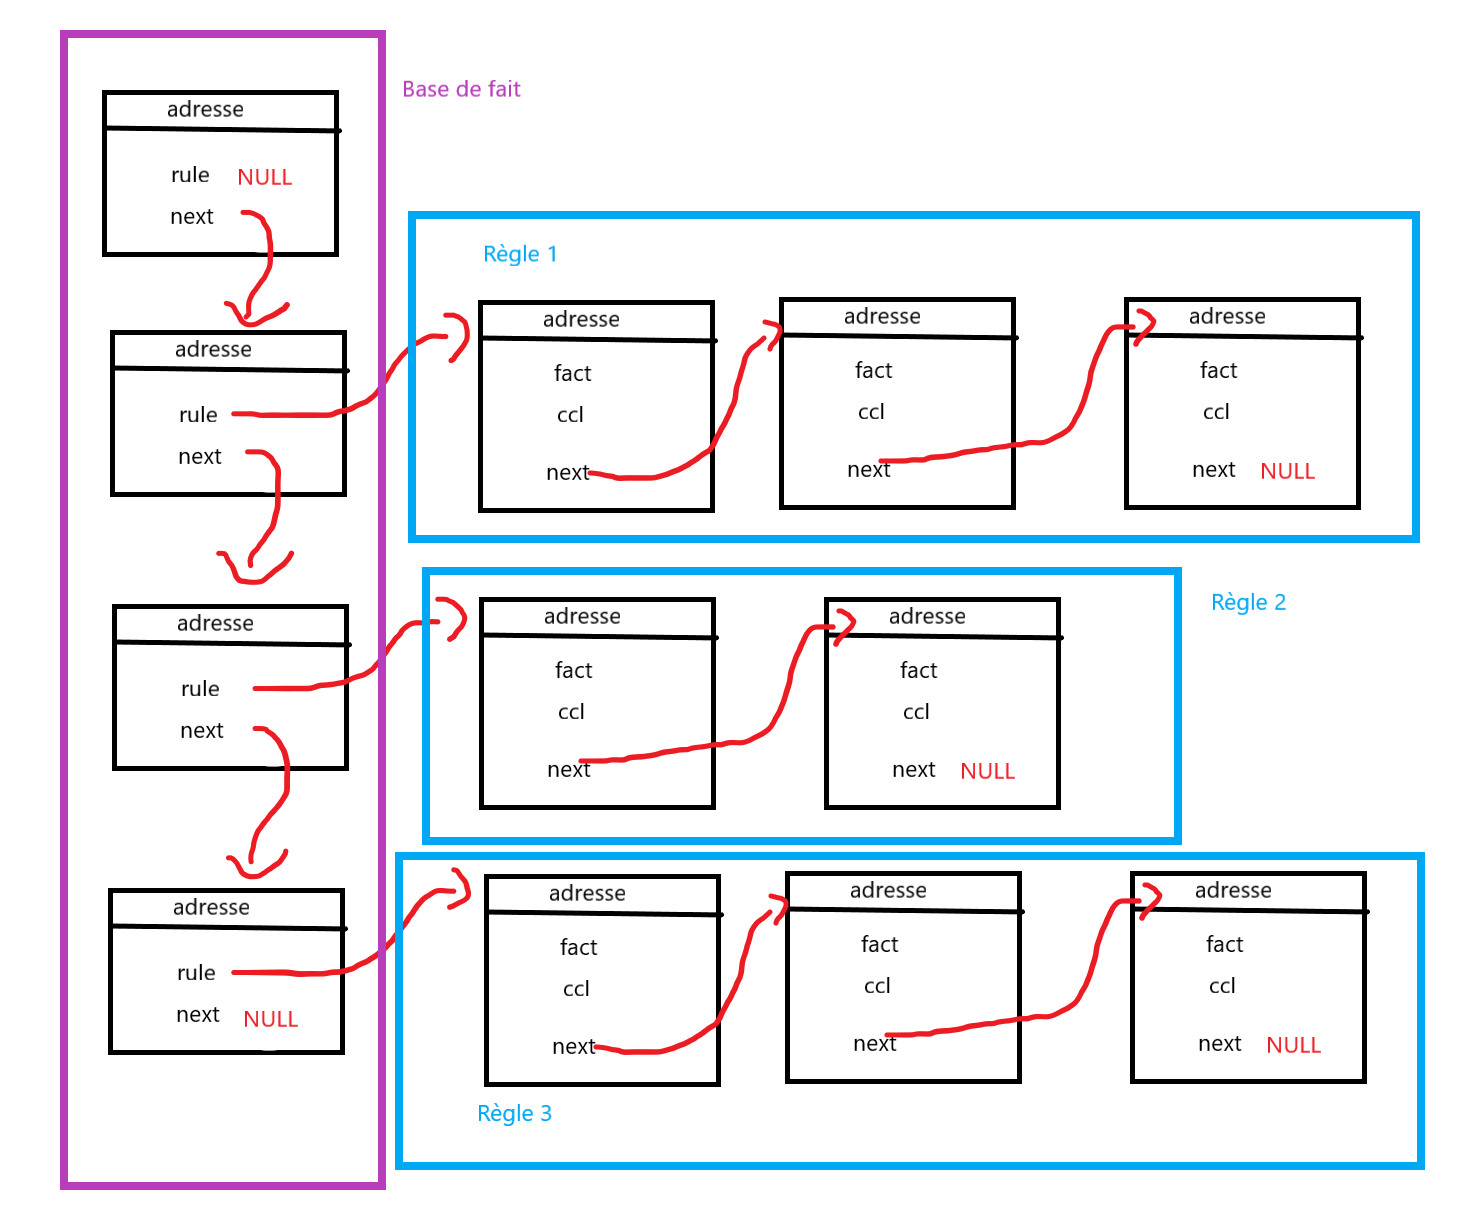
\includegraphics[width=16cm,height=114mm]{Explication.png} 

\section{Choix d'implémentation}

\newpage

\part{Algorithmes}

\newpage

\section{Règles}

\subsection{Nouvelle Règle}
L'algorithme ci-dessous permet de créer une règle vide et de retourner son pointeur.\\ 
\\
\begin{algorithm}[H]

\Vars{\Arg{$R$}{La nouvelle Règle}}

\Result{\Arg{$R$}{Règle}}

\Begin({RègleVide()}){
	\Assign{$R$}{\textit{règle\_vide}}
}
\caption{RègleVide\label{RV}}

\end{algorithm}

\subsection{Ajout de Prémisses}
L'algorithme ci-dessous permet d'ajouter une prémisse à une règle.\\
\\
\begin{algorithm}[H]

\Vars{\\
- \Arg{$P$}{Prémisse à rajouter}\\
- \Arg{$R$}{Règle dont on veut rajouter une prémisse}\\
- \Arg{$R'$}{Stockage du dernier objet d'une règle}\\
- \Arg{$T$}{Stockage de l'avant-dernier objet de la règle}\\
- \Arg{$NP$}{L'adresse de la nouvelle prémisse}}

\Data{\Arg{$R$}{Règle}}

\Result{\Arg{$R$}{Règle}}

\Begin({AjoutPrémisse ($C$,$R$)}){

\While{Suivant($R$) $\neq$ indéfini}{
	
	\Assign{$T$}{Suivant($R$)}\\
	\Assign{$R$}{Suivant($R$)}
	
}
\Assign{Conclusion($R'$)}{$R$}\\
\Assign{Fait($NP$)}{$R$}

\If{Conclusion($R'$)=1}{
	\Assign{Suivant($T$)}{$NP$}\\
	\Assign{Suivant($NP$)}{$R'$}
} \Else {
	\Assign{Suivant($R$)}{$NP$}
}
}

\caption{AjoutPrémisse\label{AP}}

\end{algorithm}

\newpage

\subsection{Créer une conclusion}
L'algorithme ci-dessous permet d'ajouter une conclusion à une règle.\\
\\
\begin{algorithm}[H]
\Vars{\\

- \Arg{$C$}{Conclusion à rajouter}\\
- \Arg{$R$}{Règle dont on veut rajouter une conclusion}\\
- \Arg{$R'$}{Règle de transit}}

\Data{\Arg{$R$}{Règle}}
\Result{\Arg{$R$}{Règle}}

\Begin({CréerConclusion ($C$,$R$)}){

\While{Suivant($R$) $\neq$ indéfini}{

	\Assign{$R$}{Suivant($R$)}
	
}
\If{Conclusion($R$) = 0}{

	\Assign{$R'$}{\textit{RègleVide()}}\\
	\Assign{Fait($R'$)}{$C$}\\
	\Assign {Conclusion($R'$)}{1}\\
	\Assign{Suivant($R$)}{$R'$}\\
	\Assign{Résultat}{Vrai}
	
}
\Else {
	\Assign{Résultat}{Faux}
}
}
\caption{CréerConclusion\label{CCL}}

\end{algorithm}

\newpage

\subsection{Test 1: Une prémisse appartient à une règle}
L'algorithme ci-dessous permet de vérifier si une règle contient une prémisse ou non, il retourne vrai si la prémisse a été trouvée et il retourne faux si cette prémisse n'est pas contenue dans la règle.\\
\\ 
\begin{algorithm}[H]

\Vars{\\
- \Arg{$R$}{Règle}\\
- \Arg{$P$}{Prémisse que l'on veut tester}}
\Data{\Arg{$R$}{Règle}}
\Result{\Arg{$Resultat$}{Boléen}}

\Begin({TestPrémisse ($P$,$R$)}){

\While{Suivant($R$) $\neq$ indéfini}{

	\If{ComparerCaractère(Fact($R$),$P$)=0}{
	
		\Assign{Résultat}{Vrai}
		
	}
	
	\Assign{$R$}{Suivant($R$)}
	
}

\If{  (Conlusion($R$)=0) \Et (ComparerCaractère(Fact($R$),$P$)=0)}{

	\Assign{Résultat}{Vrai}
	
} \Else {
	\Assign{Résultat}{Faux}
}

}

\caption{TestPrémisse\label{TP}}

\end{algorithm}

\newpage

\subsection{Supprimer une prémisse d'une règle}
L'algorithme ci-dessous permet de supprimer une prémisse d'une règle, il retourne Vrai si l'opération a pu être réalisé et retourne faux s'il n'a pas pu trouver la prémisse en question.\\
\\
\begin{algorithm}[H]

\Vars{\\
- \Arg{$P$}{Prémisse à rajouter}\\
- \Arg{$R$}{Règle dont on veut rajouter une prémisse}\\
- \Arg{$R'$}{Stockage du dernier objet d'une règle}\\
- \Arg{$T$}{Stockage de l'avant-dernier objet de la règle}\\

\Data{\Arg{$R$}{Règle}}

\Result{\Arg{$Resultat$}{Boléen}}

\Begin({SupprimerPrémisse ($P$,$R$)}){

\If {\textit{PrémisseVide($R$}=1}{

	\Assign{Résultat}{Faux}
	
}\Else{

	\While{$R$ $\neq$ indéfini}{
	
	\Assign{$T$}{$R$}\\
	
	\If{(ComparerCaractère(Fait($R$),$P$)=1) \Et (Conclusion($R$)=1)}{
	
		\Assign{Suivant($T$)}{Suivant($R$)}\\
		Libérer($R$)\\
		\Assign{Résultat}{Vrai}
	}
	\Assign{$R$}{Suivant($R$)}
	}
	\Assign{Résultat}{Faux}
}

}

}

\caption{SupprimerPrémisse\label{SP}}

\end{algorithm}

\newpage

\subsection{Test 2: Prémisse vide d'une règle}
L'algorithme ci-dessous test si une règle contient des prémisses ou non. Il retourne Vrai si la règle ne contient pas de prémisses (elle peut tout de même contenir une conclusion) et retourne faux si elle contient des prémisses.\\
\\
\begin{algorithm}[H]

\Vars{\Arg{$R$}{Règle que l'on veut tester}}
\Data{\Arg{$R$}{Règle}}
\Result{\Arg{$Resultat$}{Boléen}}

\Begin({PrémisseVide ($R$)}){

	\If{Suivant($R$) $\neq$ indéfini}{
	\Assign{Résultat}{Faux}
	}
	
	\ElseIf {Conclusion(Suivant($R$))=1}{
	\Assign{Résultat}{Vrai}	
	}
	
	\Else {
	\Assign{Résultat}{Faux}
	}
}
\caption{PrémisseVide\label{PV}}

\end{algorithm}

\subsection{Accéder à la première prémisse d'une règle}
L'algorithme ci-dessous permet de connaître la première prémisse d'une règle (si celle ci en contient bien sûr). Ce dernier retourne un pointeur lié à la première prémisse de la règle.\\
\\
\begin{algorithm}[H]

\Vars{\Arg{$R$}{Règle dont on veut voir la prémisse}}
\Data{\Arg{$R$}{Règle}}
\Result{\Arg{$P$}{Prémisse}}

\Begin({PremièrePrémisse ($R$)}){

	\While{Suivant($R$) $\neq$ indéfini}{

	\Assign{$R$}{Suivant($R$)}
	}
	\If{Conclusion($R$)=1}{
		Retourner (Fait($R$))\\
	}
		Retourner indéfini\\
}


\caption{PremièrePrémisse\label{PP}}

\end{algorithm}

\newpage

\subsection{Accéder à la conclusion d'une règle}
L'algorithme ci-dessous permet de connaître la conclusion d'une règle (si celle ci existe bien sûr). Ce dernier retourne un pointeur lié à la conclusion de la règle.\\
\\
\begin{algorithm}[H]

\Vars{\Arg{$R$}{Règle dont on veut la conclusion}}

\Data{\Arg{$R$}{Règle}}

\Result{\Arg{$P$}{Prémisse}}

\Begin({VoirConclusion ($C$,$R$)}){

\While{Suivant($R$) $\neq$ indéfini}{
	\Assign{$R$}{Suivant($R$)}	
}
\If{Conclusion(Rule)=1}{
	\Assign{$P$}{Fait($R$)}
}
\Else{
	\Assign{$P$}{indéfini}  
}
}

\caption{VoirConclusion\label{VC}}

\end{algorithm}

\newpage

\section{Base de Connaissances}

\subsection{Nouvelle Base de Connaissances}
L'algorithme ci-dessous permet de créer une base de connaissances vide. Il retourne le pointeur lié à cette base de connaissances.\\
\\
\begin{algorithm}[H]

\Vars{\Arg{$BC$}{La nouvelle Base de Connaissances}}

\Result{\Arg{$BC$}{Base de Connaissances}}

\Begin({BC\_Vide()}){
	\Assign{$BC$}{\textit{BC\_vide}}
}

\caption{BC\_Vide\label{BC}}

\end{algorithm}

\subsection{Ajouter une nouvelle règle}
L'algorithme ci-dessous permet d'ajouter à une base de connaissances existante une nouvelle règle. Il retourne vrai si l'opération s'est déroulé avec succès.\\
\\
\begin{algorithm}[H]

\Vars{\\
- \Arg{$R$}{Règle à rajouter}\\
- \Arg{$BC$}{Base dont on veut rajouter une règle}\\
- \Arg{$NR$}{Nouvelle règle}\\}

\Data{\Arg{$BC$}{Base de Connaissances}}

\Result{\Arg{$Resultat$}{Boléen}}

\Begin({AjoutRègle ($R$,$BC$)}){

\Assign{$NR$}{\textit{BC\_Vide()}}\\

\While{Suivant($BC$) $\neq$ indéfini}{
	
	\Assign{$BC$}{Suivant($BC$)}
}

\Assign{Suivant($BC$)}{$NR$}\\
\Assign{Règle($NR$)}{$R$}\\
Retourner Vrai

}

\caption{AjoutRègle\label{AR}}

\end{algorithm}

\newpage

\subsection{Afficher la première règle}
L'algorithme ci-dessous permet d'afficher la première règle d'une base de connaissance. Il retourne le pointeur lié à la première règle de la base (si celle-ci existe).\\
\\
\begin{algorithm}[H]

\Vars{\Arg{$BC$}{La base de connaissances en question}}

\Result{\Arg{$R$}{Règle}}

\Begin({PremièreRègle($BC$)}){

	\If{Suivant($BC$) = indéfini}{
	
	Retourner indéfini\\
	}\Else {
	Retourner Règle(Suivant($BC$))\\
	}
}

\caption{PremièreRègle\label{PR}}

\end{algorithm}

\newpage

\section{Moteur d'Inférence}

\subsection{Moteur d'Inférence}
L'algorithme ci-dessous retourne une liste chaînée des faits vrais.\\
\\
\begin{algorithm}[H]

\Vars{\\
-\Arg{$LF$}{Liste de Faits}\\
-\Arg{$BC$}{Base connaissances}\\
-\Arg{$KB$}{Base de connaissances transitoire}\\
-\Arg{$PF$}{Liste de faits transitoires}\\
-\Arg{$RF$}{Liste de faits transitoire}\\
}
\Data{\Arg{$LF$}{Liste de faits}}
\Result{\Arg{$R$}{Règle}}

\Begin({MoteurInférence($BC$,$LF$)}){
	
	\While{$PF$ $\neq$ indéfini}{
	\textit{AjouterFaitsListe($PF$,$F$)}\\
	\Assign{$PF$}{Suivant($PF$)}
	}
	
	\While{$KB$ $\neq$ indéfini}{
	\If{\textit{RègleVraie(Règle($KB$),$RF$)}=Vrai}{
	\textit{AjouterFaitsListe(VoirConclusion(Rule($KB$),$RF$)}
	}
	\Assign{$KB$}{Suivant($KB$)}
	}
	Retourner $RF$\\
}

\caption{MoteurInférence\label{MI}}

\end{algorithm}

\newpage

\subsection{Règle Vraie}
L'algorithme ci-dessous permet de savoir si une règle est vraie. Il retourne indéfini si la règle est fausse et la conclusion si la règle est vraie\\
\\
\begin{algorithm}[H]

\Vars{\\
-\Arg{$LF$}{Une liste de faits}\\
-\Arg{$R$}{Une règle}}
\Data{\Arg{$LF$}{Une liste de faits}\Arg{$R$}{Une règle}}
\Result{\Arg{$Resultat$}{Un fait}}

\Begin({RègleVraie($BC$)}){

	\If{(\textit{PrémisseVide($R$)} = Faux) \Et (\textit{VoirConclusion($R$)} $\neq$ indéfini) }{
	
	\While{Suivant($R$) $\neq$ indéfini}{
	\If{\textit{PrémisseVraie(Fait($R$),$LF$)}=Faux}{
	Retourner indéfini\\
	}
	\Assign{$R$}{Suivant($R$)}
	}
	Retourner Fait($R$)\\
}\Else {
	Retourner indéfini\\
	}
}
\caption{RègleVraie\label{RV}}

\end{algorithm}

\newpage

\subsection{Prémisse Vraie}
L'algorithme ci-dessous permet de tester si une prémisse est vraie. Il retourne vrai si la prémisse est vraie et faux si la prémisse est fausse.\\
\\
\begin{algorithm}[H]

\Vars{\\
-\Arg{$LF$}{La liste de faits}\\
-\Arg{$F$}{Un fait}}

\Data{\Arg{$LF$}{Liste de faits}}

\Result{\Arg{$Resultat$}{Boléen}}

\Begin({PrémisseVraie($F$,$LF$)}){

	\While{Suivant($LF$) $\neq$ indéfini}{
	\If{ComparerCaractère(Fait($LF$),$F$)=0}{
	Retourner Vrai\\
	}
	\Assign{$LF$}{Suivant($LF$)}
	}
	\If{ComparerCaractère(Fait($LF$),$F$)=0}{
	Retourner Vrai\\
	}
	\Else {
	Retourner Faux\\
	}
}

\caption{PrémisseVraie\label{PV}}

\end{algorithm}

\subsection{Ajouter un fait à une liste}
L'algorithme ci-dessous\\
\\
\begin{algorithm}[H]

\Vars{\Arg{$BC$}{La base de connaissances en question}}

\Result{\Arg{$R$}{Règle}}

\Begin({PremièreRègle($BC$)}){

	\If{Suivant($BC$) = indéfini}{
	
	Retourner indéfini\\
	}\Else {
	Retourner Règle(Suivant($BC$))\\
	}
}

\caption{PremièreRègle\label{PR}}

\end{algorithm}

\newpage

\part{Jeux d'essais}

\newpage

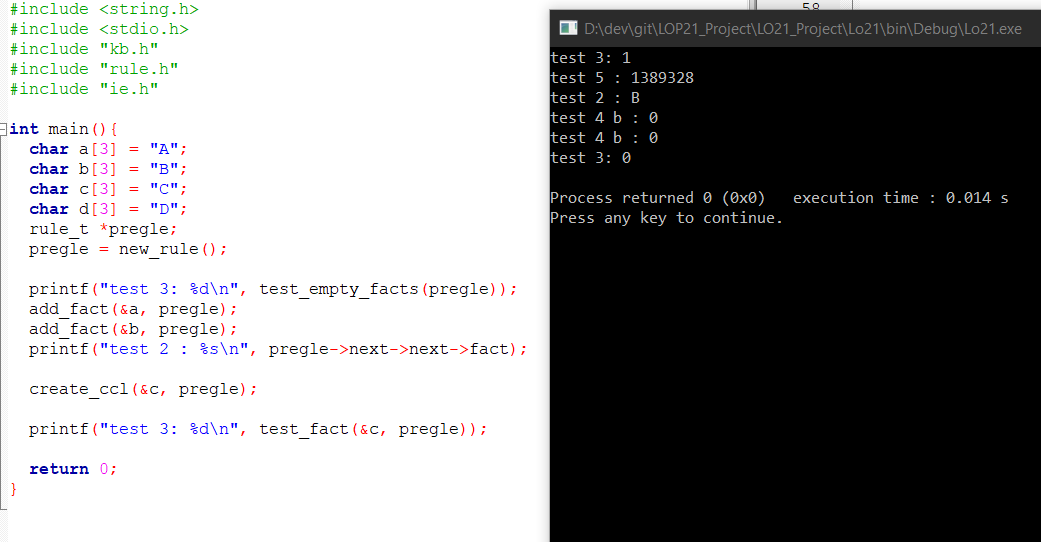
\includegraphics[width=16cm,height=114mm]{JeuEssai1.png} 

\newpage

\part{Commentaires sur les résultats}

\newpage

\end{document}